\documentclass{ltxdoc}
\usepackage[show]{cloze}
\usepackage{graphicx}
\usepackage{paralist}
\usepackage{titlesec}
\usepackage{mdframed}
\titleformat{\paragraph}[hang]{%
  \normalfont\normalsize\bfseries%
  }{\theparagraph}{1em}{}
\titleformat{\subparagraph}[hang]{%
  \normalfont\small\bfseries%
  }{\thesubparagraph}{1em}{}
  \titlespacing*{\subparagraph}{0pt}{*1}{0pt}

\usepackage[
  colorlinks=true,
  linkcolor=red,
  filecolor=red,
  urlcolor=red,
]{hyperref}

\usepackage{minted}
\usemintedstyle{colorful}
\BeforeBeginEnvironment{minted}{\begin{mdframed}[backgroundcolor=gray!3]}
\AfterEndEnvironment{minted}{\end{mdframed}}
\setminted{
  breaklines=true,
  fontsize=\footnotesize,
}

\MakeShortVerb{\|}

\setlength{\fboxrule}{0.2pt}
\setlength{\fboxsep}{4pt}

\makeatletter
\newcommand{\@minipagerestore}{\setlength{\parindent}{10pt}}
\makeatother

\newmdenv{example}
\definecolor{graybackground}{gray}{0.97}
\surroundwithmdframed[backgroundcolor=graybackground]{verbatim}

\newcommand{\getdefaults}[1]{%
  \directlua{tex.print(cloze.get_defaults('#1'))}%
}

\newcommand{\expdesc}[1]{(|#1|)}

\newcommand{\desc}[1]{%
  \hfill%
  \expdesc{#1}%
  \par%
}

\def\tt#1{\texttt{#1}}

\def\secref#1{(\rightarrow\ \ref{#1})}

\newcommand{\option}[2]{\tt{[#1=}\meta{#2}\tt{]}}
\newcommand{\clozeluafunction}[1]{
  \marginpar{%
    \raggedleft%
    \MacroFont%
    \tt{%
      \scantokens{\catcode`\_=12\relax#1}%
    }%
  }%
}

\newcommand{\nodelisthfont}{\bfseries\sffamily}

\newcommand{\nodelistheader}{
  \hline
  \nodelisthfont Variable name &
  \nodelisthfont Node type &
  \nodelisthfont Node subtype &
  \nodelisthfont Parameter \\
  \hline
}

\newenvironment{nodelist}{
  \noindent
  \begingroup
  \footnotesize
  \begin{tabular}{llll}
  \nodelistheader
}{
  \hline
  \end{tabular}
  \endgroup
}

\EnableCrossrefs
\CodelineIndex
\RecordChanges
\begin{document}

\providecommand*{\url}{\texttt}
\GetFileInfo{cloze.dtx}
\title{The \cloze{cloze} package%
  \thanks{Many thanks to Robert-Michael Huber for his advice
and to Paul Isambert for his article \emph{"Three things you can do with
Lua\TeX{} that would be extremely painful otherwise"} in TUGboat, Volume
31 (2010), No. 3. This article helped a lot to write this package.}%
}
\author{%
  Josef Friedrich\\%
  \url{josef@friedrich.rocks}\\%
  \href{https://github.com/Josef-Friedrich/cloze}{github.com/Josef-Friedrich/cloze}%
}
\date{v.1.5~from 2020/05/07}

\maketitle\vfill

\pagebreak

\setcounter{secnumdepth}{5}
\setcounter{tocdepth}{5}
\tableofcontents

%-----------------------------------------------------------------------
% Introduction
%-----------------------------------------------------------------------

\pagebreak
\section{Introduction}

\emph{cloze} is a plain \TeX{} or a \LaTeX{} package to generate cloze
texts. It uses the capabilities of the modern \TeX{} engine
\emph{Lua\TeX}. Therefore, you must use Lua\TeX{} or Lua\LaTeX{} to
create documents containing gaps.

\begin{center}
\begin{minipage}{0.4\linewidth}
\begin{verbatim}
lualatex cloze-text.tex
\end{verbatim}
\end{minipage}
or
\begin{minipage}{0.4\linewidth}
\begin{verbatim}
luatex cloze-text.tex
\end{verbatim}
\end{minipage}
\end{center}

\noindent
The main feature of the package is that the formatting doesn't change
when using the |hide| and |show| \secref{sec:option-hide} options.

\newcommand{\clozelorem}{%
Lorem ipsum \cloze{dolor sit} amet, consectetur \cloze{adipisicing}
elit, sed do eiusmod tempor incididunt ut labore et \cloze{dolore magna}
aliqua. Ut enim ad minim veniam, quis nostrud \cloze{exercitation}
ullamco laboris nisi ut \cloze{aliquip} ex ea commodo consequat.%
}

\begin{example}
\clozelorem
\end{example}

\clozeset{hide}

\noindent
The command |\clozeset{hide}| only shows gaps. When you put both texts
on top of each other you will see that they perfectly match.

\begin{example}
\clozelorem
\end{example}

\clozeset{show}

%-----------------------------------------------------------------------
% Usage
%-----------------------------------------------------------------------

\section{Usage}

%-----------------------------------------------------------------------
%
%-----------------------------------------------------------------------

\subsection{Interfaces}

The main difference between the plain \TeX{} and the \LaTeX{} interface
is option handling. In \LaTeX{} options can be set using a key-value
pairs. In plain \TeX{} the only possibility to set options in plain
\TeX{} is using the \cmd{\clozesetoption} \secref{sec:cmd-clozesetoption}.

%%
%
%%

\subsubsection{The plain \TeX{} interface}

\begin{minted}{tex}
\input cloze.tex
\clozesetoption{margin}{1cm}
\clozeshow
Lorem \cloze{ipsum} dolor.
\bye
\end{minted}

%%
%
%%

\subsubsection{The \LaTeX{} interface}

\begin{minted}{latex}
\documentclass{article}
\usepackage[show,margin=1cm]{cloze}
\begin{document}
Lorem \cloze{ipsum} dolor.
\end{document}
\end{minted}

\subsection{The commands and environments}

There are the commands
\cmd{\cloze},
\cmd{\clozefix},
\cmd{\clozefil},
\cmd{\clozenol},
\cmd{\clozeparcmd},
\cmd{\clozestrike} and the environments
|clozepar| and
|clozebox|
to generate cloze texts.

%%
% \cloze
%%

\subsubsection{\cmd{\cloze}}
\label{sec:command-cloze}

\DescribeMacro{\cloze} \cmd{\cloze}\oarg{options}\marg{some text}: The
command \cmd{\cloze} is similar to a command that offers the possibility
to underline the texts. \cmd{\cloze} does not prevent line breaks. The
width of a gap depends on the number of letters and the font used.
The only option which affects the widths of a gap is the option
|margin| \secref{sec:option-margin}.

\begin{example}
Lorem ipsum \cloze{dolor} sit amet, \cloze{consectetur} adipisicing
elit, sed do eiusmod tempor incididunt ut labore et dolore
\cloze{magna aliqua. Ut enim ad minim veniam, quis nostrud exercitation
ullamco laboris nisi} ut aliquip ex ea commodo consequat.
\end{example}

\noindent It is possible to convert a complete paragraph into a `gap'.
But don't forget: There is a special environment for this: \tt{clozepar}
\secref{sec:command-clozepar}.

\begin{example}
\cloze{Lorem ipsum dolor sit amet, consectetur adipisicing elit, sed do
eiusmod tempor incididunt ut labore et dolore magna aliqua. Ut enim ad
minim veniam, quis nostrud exercitation ullamco laboris nisi ut aliquip
ex ea commodo consequat.}
\end{example}

\noindent The command \cmd{\cloze} doesn't change the behavior of the
hyphenation. Let's try some long German words:

\begin{example}
es
\cloze{Te\-le\-kom\-mu\-ni\-ka\-tions\-ü\-ber\-wach\-ung}
geht
\cloze{Un\-ter\-neh\-mens\-steu\-er\-fort\-ent\-wick\-lungs\-ge\-setz}
\cloze{Ab\-teil\-ungs\-lei\-ter\-in}
\cloze{Ober\-kom\-mi\-sar\-in}
auch
\cloze{Fil\-lial\-lei\-ter\-in}
kurz.
\end{example}

%%
% \clozesetfont
%%

\subsubsection{\cmd{\clozesetfont}}
\label{sec:command-clozesetfont}
\label{sec:command-clozefont}

\DescribeMacro{\clozesetfont}
The gap font can be changed by using the command
\cmd{\clozesetfont}. \tt{\string\cloze\-set\-font} redefines the command
\cmd{\clozefont} which contains the font definition.
Thus, the command \tt{\string\clozesetfont\string{\string\Large\string}}
has the same effect as
|\def\clozefont{\Large}|

\clozesetfont{\Large}

\begin{example}
Excepteur \cloze{sint} occaecat \cloze{cupidatat} non proident.
\end{example}

\noindent Please do not put any color definitions in
\cmd{\clozesetfont}, as it won't work. Use the option
|textcolor| instead \secref{sec:option-textcolor}.

|\clozesetfont{\ttfamily\normalsize}| changes the gap text for example
into a normal sized typewriter font.

\clozesetfont{\ttfamily\normalsize}

\begin{example}
Excepteur \cloze{sint} occaecat \cloze{cupidatat} non proident.
\end{example}

\clozesetfont{\itshape}

%%
% \clozefix
%%

\subsubsection{\cmd{\clozefix}}
\label{sec:command-clozefix}

\DescribeMacro{\clozefix} \cmd{\clozefix}\oarg{options}\marg{some text}:
The command \cmd{\clozefix} creates gaps with a fixed width. The
clozes are default concering the width \tt{\getdefaults{width}}.

\begin{example}
\noindent Lorem ipsum dolor sit amet:
\begin{compactenum}
\item \clozefix[width=5cm]{consectetur}
\item \clozefix[width=5cm]{adipisicing}
\item \clozefix[width=5cm]{elit}
\end{compactenum}
sed do eiusmod.
\end{example}

Gaps with a fixed width are much harder to solve.

\begin{example}
Lorem ipsum dolor \clozefix[align=center,width=3cm]{sit} amet,
\clozefix[align=center,width=3cm]{consectetur} adipisicing elit, sed do
eiusmod tempor incididunt \clozefix[align=center,width=3cm]{ut} labore
et dolore magna aliqua.
\end{example}

Using the option |align| you can make nice tabulars like this:

\begin{example}
\begin{tabular}{p{5cm}p{4cm}}
\raggedleft Composer & Life span \\
\clozefix[width=5cm,align=right]{Joseph Haydn} & \clozefix{1723-1809} \\
\clozefix[width=5cm,align=right]{Wolfgang Amadeus Mozart} & \clozefix{1756-1791} \\
\clozefix[width=5cm,align=right]{Ludwig van Beethoven} & \clozefix{1770-1827} \\
\end{tabular}
\end{example}

%%
% \clozenol
%%

\subsubsection{\cmd{\clozenol}}
\label{sec:command-clozenol}
\DescribeMacro{\clozenol} \cmd{\clozenol}\oarg{options}\marg{some text}:
The macro name |clozenol| stands for \emph{“cloze no line”}. As the
the name suggests this macro typesets cloze texts without a line.
\cmd{\clozenol} is a convenient abbreviation for
|\cloze[thickness=0pt]{text}|.

\begin{minted}{latex}
Lorem \clozenol{ipsum dolor} sit amet.
\end{minted}

\begin{example}
Lorem \clozenol{ipsum dolor} sit amet.
\end{example}

\begin{minted}{latex}
Lorem \clozenol[textcolor=green]{ipsum dolor} sit amet.
\end{minted}

\begin{example}
Lorem \clozenol[textcolor=green]{ipsum dolor} sit amet.
\end{example}

\noindent
The next examples are showing that \cmd{\clozenol} behaves exactly as
\cmd{\clozenol} with the option |thickness=0pt|
(|\cloze[thickness=0pt]|) set: The text layout doesn’t change if we are
hiding the gaps and the hidden text is not really hidden. It is removed.
It can not be copied.

\begin{mdframed}[backgroundcolor=gray!40]
Lorem ipsum \clozenol{dolor sit amet, consetetur sadipscing elitr, sed
diam nonumy eirmod tempor invidunt ut labore et dolore magna aliquyam
erat, sed diam voluptua} sit amet.
\end{mdframed}

\noindent
Now hide the text

\clozehide

\begin{mdframed}[backgroundcolor=gray!40]
Lorem ipsum \clozenol{dolor sit amet, consetetur sadipscing elitr, sed
diam nonumy eirmod tempor invidunt ut labore et dolore magna aliquyam
erat, sed diam voluptua} sit amet.
\end{mdframed}

\clozeshow

%%
% \clozefil
%%

\subsubsection{\cmd{\clozefil}}
\label{sec:command-clozefil}

\DescribeMacro{\clozefil} \cmd{\clozefil}\oarg{options}\marg{some text}:
The name of the command is inspired by \cmd{\hfil}, \cmd{\hfill}, and
\cmd{\hfilll}. Only \cmd{\clozefil} fills out all available horizontal
spaces with a line.

\begin{example}
Lorem ipsum dolor sit amet, \clozefil{consectetur adipisicing elit, sed
do eiusmod.}

Ut enim \clozefil{ad minim veniam} exercitation.
\end{example}

%%
% \clozeextend
%%

\subsubsection{\cmd{\clozeextend}}
\label{sec:command-clozeextend}

\DescribeMacro{\clozeextend} \cmd{\clozeextend}\oarg{spaces}:
The command |\clozeextend| adds some invisible placeholders to extend
some cloze texts with blank space.

\begin{minted}{latex}
\begin{itemize}
\item \clozefil{Lorem ipsum dolor sit amet, consectetur adipisicing
elit, sed do eiusmod tempor incididunt ut labore et dolore magna
aliqua.}
\item \clozefil{Ut enim ad minim veniam \clozeextend[20]}
\item \clozefil{quis nostrud \clozeextend[20]}
\end{itemize}
\end{minted}

\begin{example}
\begin{itemize}
\item \clozefil{Lorem ipsum dolor sit amet, consectetur adipisicing
elit, sed do eiusmod tempor incididunt ut labore et dolore magna
aliqua.}
\item \clozefil{Ut enim ad minim veniam \clozeextend[20]}
\item \clozefil{quis nostrud \clozeextend[20]}
\end{itemize}
\end{example}

%%
% clozepar
%%

\subsubsection{\tt{clozepar}}
\label{sec:command-clozepar}

\DescribeEnv{clozepar} |\begin{clozepar}|\oarg{options} \dots
\textit{some text} \dots |\end{clozepar}|: The environment \tt{clozepar}
transforms a complete paragraph into a cloze text. The options |align|,
|margin| and |width| have no effect on this environment.

\begin{example}
Lorem ipsum dolor sit amet, consectetur adipisicing elit ullamco laboris
nisi.

\begin{clozepar}
Ut enim ad minim veniam, quis nostrud exercitation ullamco laboris nisi
ut aliquip ex ea commodo consequat. Duis aute irure dolor in
reprehenderit in voluptate velit esse cillum.
\end{clozepar}

Excepteur sint occaecat cupidatat non proident.
\end{example}

%%
% \clozeparcmd
%%

\subsubsection{\cmd{\clozeparcmd}}
\label{sec:command-clozeparcmd}
\DescribeMacro{\clozeparcmd} \cmd{\clozeparcmd}: The command
\cmd{\clozeparcmd} is the macro version of the environment |clozepar|.

%%
% clozebox
%%

\subsubsection{\tt{clozebox}}
\label{sec:command-clozebox}

\DescribeEnv{clozebox} |\begin{clozebox}|*\oarg{options} \dots
\textit{some text} \dots |\end{clozebox}|: The environment \tt{clozebox}
surrounds a text with a box. The starred version omits the line
around the box. Use the options |boxwidth| and |boxheight| to specify
the dimensions of the box. By default the width of the box is
|\linewidth|.

\begin{minted}{latex}
\begin{clozebox}
Lorem ipsum dolor sit amet, consectetur adipisicing elit, sed do eiusmod
tempor incididunt ut labore et dolore magna aliqua.
\end{clozebox}
\end{minted}

\bigskip
\noindent
|\clozehide|
\clozehide
\bigskip

\begin{center}
\begin{clozebox}[boxwidth=8cm]
Lorem ipsum dolor sit amet, consectetur adipisicing elit, sed do eiusmod
tempor incididunt ut labore et dolore magna aliqua.
\end{clozebox}
\end{center}

\bigskip
\noindent
|\clozeshow|
\clozeshow
\bigskip

\begin{center}
\begin{clozebox}[boxwidth=8cm]
Lorem ipsum dolor sit amet, consectetur adipisicing elit, sed do eiusmod
tempor incididunt ut labore et dolore magna aliqua.
\end{clozebox}
\end{center}

\paragraph{Option boxwidth}
\label{sec:command-clozebox-boxwidth}
See the documentation about the option \secref{sec:option-boxwidth}.

\begin{minted}{latex}
\begin{clozebox}[boxwidth=5cm]
Lorem ipsum dolor sit amet, consectetur adipisicing elit, sed do eiusmod
tempor incididunt ut labore et dolore magna aliqua.
\end{clozebox}
\end{minted}

\begin{center}
\begin{clozebox}[boxwidth=5cm]
Lorem ipsum dolor sit amet, consectetur adipisicing elit, sed do eiusmod
tempor incididunt ut labore et dolore magna aliqua.
\end{clozebox}
\end{center}

\paragraph{Option boxheight}
\label{sec:command-clozebox-boxheight}
See the documentation about the option \secref{sec:option-boxheight}.

\begin{minted}{latex}
\begin{clozebox}[boxwidth=5cm,boxheight=5cm]
Lorem ipsum dolor sit amet, consectetur adipisicing elit, sed do eiusmod
tempor incididunt ut labore et dolore magna aliqua.
\end{clozebox}
\end{minted}

\begin{center}
\begin{clozebox}[boxwidth=5cm,boxheight=5cm]
Lorem ipsum dolor sit amet, consectetur adipisicing elit, sed do eiusmod
tempor incididunt ut labore et dolore magna aliqua.
\end{clozebox}
\end{center}

\paragraph{starred}

% starred
\begin{minted}{latex}
\begin{clozebox}*[boxwidth=5cm,boxheight=5cm]
Lorem ipsum dolor sit amet, consectetur adipisicing elit, sed do eiusmod
tempor incididunt ut labore et dolore magna aliqua.
\end{clozebox}
\end{minted}

\begin{center}
\begin{clozebox}*[boxwidth=5cm,boxheight=5cm]
Lorem ipsum dolor sit amet, consectetur adipisicing elit, sed do eiusmod
tempor incididunt ut labore et dolore magna aliqua.
\end{clozebox}
\end{center}

%%
% clozespace
%%

\subsubsection{\tt{clozespace}}
\label{sec:command-clozespace}

\DescribeEnv{clozespace} |\begin{clozespace}|\oarg{options} \dots
\textit{some text} \dots |\end{clozespace}|

\begin{minted}{latex}
\begin{clozespace}[spacing=2]
\clozesetfont{\ttfamily\Huge}
Lorem \cloze{ipsum} dolor sit \cloze{amet}, consectetur adipisicing
elit, sed do eiusmod tempor incididunt ut labore et dolore magna
aliqua. Ut enim ad minim veniam, quis \cloze{nostrud}
exercitation ullamco \cloze{laboris} nisi ut aliquip ex ea commodo
consequat.
\end{clozespace}
\end{minted}

\begin{example}
\begin{clozespace}[spacing=2]
\clozesetfont{\ttfamily\Huge}
Lorem \cloze{ipsum} dolor sit \cloze{amet}, consectetur adipisicing
elit, sed do eiusmod tempor incididunt ut labore et dolore magna
aliqua. Ut enim ad minim veniam, quis \cloze{nostrud}
exercitation ullamco \cloze{laboris} nisi ut aliquip ex ea commodo
consequat.
\vspace{-0.8cm}
\end{clozespace}
\end{example}

%%
% \clozeline
%%

\subsubsection{\cmd{\clozeline}}
\label{sec:command-clozeline}

\DescribeMacro{\clozeline}
\cmd{\clozeline}\oarg{options}:
To create a cloze line of a certain width, use the command
\cmd{\clozeline}. The default width of the line is
\tt{\getdefaults{width}}. In combination with the other cloze commands
you can create for example an irregular alignment of the cloze text.

\begin{minted}{latex}
Ut enim ad
\clozeline[width=1cm]\cloze{minim}\clozeline[width=3cm]
minim veniam
\end{minted}

\begin{example}
Ut enim ad \clozeline[width=1cm]\cloze{minim}\clozeline[width=3cm] minim
veniam,
\end{example}

%%
% \clozelinefil
%%

\subsubsection{\cmd{\clozelinefil}}
\label{sec:command-clozelinefil}

\DescribeMacro{\clozelinefil}
\cmd{\clozelinefil}\oarg{options}:
This command \cmd{\clozelinefil} fills the
complete available horizontal space with a line. Moreover,
\cmd{\clozelinefil} was used to create \cmd{\clozefil}.

\begin{example}
Lorem\clozelinefil
\end{example}

%%
% \clozestrike
%%

\subsubsection{\cmd{\clozestrike}}
\label{sec:command-clozelinefil}

\DescribeMacro{\clozestrike}
\cmd{\clozestrike}\oarg{options}\marg{wrong text}\marg{correct text}

\begin{minted}{latex}
Lorem \clozestrike{ipsum}{dolor} sit amet.
\end{minted}

\begin{example}
Lorem \clozestrike{ipsum}{dolor} sit amet.
\end{example}

\begin{minted}{latex}
Lorem \clozestrike[textcolor=red]{ipsum}{dolor} sit amet.
\end{minted}

\begin{example}
Lorem \clozestrike[textcolor=red]{ipsum}{dolor} sit amet.
\end{example}

\begin{example}
\begin{clozespace}
invidunt ut \clozestrike{labore}{et dolore magna aliquyam erat}, sed
diam voluptua. At \clozestrike{vero eos}{et accusam et justo} duo
dolores et ea \clozestrike{rebum. Stet}{clita kasd gubergren}, no sea
takimata sanctus est Lorem ipsum dolor sit amet. Lorem ipsum
\clozestrike{dolor sit amet, consetetur }{sadipscing elitr, sed diam}
nonumy eirmod tempor invidunt ut labore et dolore magna
aliquyam erat, \clozestrike{sed diam voluptua}{At vero}.
\end{clozespace}
\end{example}

\begin{example}
\clozehide
\begin{clozespace}
invidunt ut \clozestrike{labore}{et dolore magna aliquyam erat}, sed
diam voluptua. At \clozestrike{vero eos}{et accusam et justo} duo
dolores et ea \clozestrike{rebum. Stet}{clita kasd gubergren}, no sea
takimata sanctus est Lorem ipsum dolor sit amet. Lorem ipsum
\clozestrike{dolor sit amet, consetetur }{sadipscing elitr, sed diam}
nonumy eirmod tempor invidunt ut labore et dolore magna
aliquyam erat, \clozestrike{sed diam voluptua}{At vero}.
\end{clozespace}
\clozeshow
\end{example}

%-----------------------------------------------------------------------
% Options
%-----------------------------------------------------------------------

\subsection{The options}

%%
% Local and global options
%%

\subsubsection{Local and global options}

The \emph{cloze} package distinguishs between \emph{local} and
\emph{global} options. Besides the possiblity to set \emph{global}
options in the \cmd{\usepackage}\oarg{global options}\marg{cloze}
declaration, the cloze package offers a special command to set
\emph{global} options:
\cmd{\clozeset}\marg{global options}

%%
% \clozesetoption
%%

\subsubsection{\cmd{\clozesetoption}}
\label{sec:command-clozesetoption}

\DescribeMacro{\clozesetoption}
\cmd{\clozesetoption}\marg{key}\marg{value}: Set a single option. In
plain \TeX{} the command sets the options only in the global option
space.

%%
% \clozeset
%%

\subsubsection{\cmd{\clozeset}}
\label{sec:command-clozeset}

\DescribeMacro{\clozeset}
\cmd{\clozeset}\marg{global options}: The command can set \emph{global}
options for each paragraph.

\begin{minted}{latex}
\clozeset{textcolor=red} Lorem \cloze{ipsum} dolor \par
\clozeset{textcolor=green} Lorem \cloze{ipsum} dolor
\end{minted}

\begin{example}
\clozeset{textcolor=red} Lorem \cloze{ipsum} dolor \par
\clozeset{textcolor=green} Lorem \cloze{ipsum} dolor
\end{example}

\noindent \cmd{\clozeset} does not change the options within a
paragraph. As you can see in the example below the last \cmd{\clozeset}
applies the color green for both gaps.

\begin{minted}{latex}
\clozeset{textcolor=red} Lorem \cloze{ipsum} dolor
\clozeset{textcolor=green} Lorem \cloze{ipsum} dolor
\end{minted}

\begin{example}
\clozeset{textcolor=red} Lorem \cloze{ipsum} dolor
\clozeset{textcolor=green} Lorem \cloze{ipsum} dolor
\end{example}

\clozereset

%%
% \clozereset
%%

\subsubsection{\cmd{\clozereset}}
\label{sec:command-clozereset}

\DescribeMacro{\clozereset}
\cmd{\clozereset}: The command resets all \emph{global} options to the
default values. It has no effect on the \emph{local} options.

\begin{minted}{latex}
\clozeset{
  thickness=3mm,
  linecolor=yellow,
  textcolor=magenta,
  margin=-2pt
}
\end{minted}

\clozeset{thickness=3mm,linecolor=yellow,textcolor=magenta,margin=-2pt}

\begin{example}
Very \cloze{silly} global \cloze{options}.
\end{example}

\begin{minted}{latex}
\clozereset
\end{minted}
\clozereset

\begin{example}
\cloze{Relax!} We can reset \cloze{those} options.
\end{example}

%%
% \clozereset
%%

\subsubsection{\cmd{\clozeshow} and \cmd{\clozehide}}
\label{sec:command-clozeshow}
\label{sec:command-clozehide}

\DescribeMacro{\clozeshow} \DescribeMacro{\clozehide}
\cmd{\clozeshow} and \cmd{\clozehide}: This commands are shortcuts for
\cmd{\clozeset}\marg{show} and \cmd{\clozeset}\marg{hide}.

\begin{minted}{latex}
\clozehide
\end{minted}
\clozehide

\begin{example}
Lorem \cloze{ipsum dolor sit} amet, consectetur \cloze{adipisicing}
elit.
\end{example}

\begin{minted}{latex}
\clozeshow
\end{minted}
\clozeshow

\begin{example}
Lorem \cloze{ipsum dolor sit} amet, consectetur \cloze{adipisicing}
elit.
\end{example}

%%
% align
%%

\subsubsection{\tt{align}}
\label{sec:option-align}

\option{align}{left/center/right}:
Only the macro \cmd{\clozefix} \secref{sec:command-clozefix} takes the
option \tt{align} into account. Possible values are \tt{left},
\tt{center} and \tt{right}. This option only makes sense, if the width
of the line is larger than the width of the text.

\newcommand{\optionsalign}[1]{%
  \noindent%
  \clozefix[align=#1,width=8cm]{Lorem ipsum}%
  \desc{#1}%
}

\begin{example}
\optionsalign{left}
\optionsalign{center}
\optionsalign{right}
\end{example}

%%
% boxheight
%%

\subsubsection{\tt{boxheight}}
\label{sec:option-boxheight}

|boxheight| specifies the height of a cloze box. This option has only
an effect on the environment |clozebox| \secref{sec:command-clozebox}.
An example can be found in the section about the environment
\secref{sec:command-clozebox-boxheight}.

%%
% boxwidth
%%

\subsubsection{\tt{boxwidth}}
\label{sec:option-boxwidth}

|boxwidth| specifies the width of a cloze box. This option has only
an effect on the environment |clozebox| \secref{sec:command-clozebox}.
An example can be found in the section about the environment
\secref{sec:command-clozebox-boxwidth}.

%%
% distance
%%

\subsubsection{\tt{distance}}
\label{sec:option-distance}

\option{distance}{dimen}:
The option |distance| specifies the spacing between the baseline of the
text and the gap line. The larger the dimension of the option
|distance|, the more moves the line down. Negative values cause the line
to appear above the baseline. The default value is
\tt{\getdefaults{distance}}.

\newcommand{\optiondistance}[1]{%
  \noindent%
  \clozefil[distance=#1]{Lorem ipsum dolor sit amet.}
  \expdesc{#1}
  \par%
}

\begin{example}
\optiondistance{\getdefaults{distance}}
\optiondistance{3pt}
\optiondistance{-3pt}
\end{example}

%%
% hide and show
%%

\subsubsection{\tt{hide} and \tt{show}}
\label{sec:option-hide}
\label{sec:option-show}

\tt{[hide]} and \tt{[show]}:
By default the cloze text is displayed. Use the option |hide| to remove
the cloze text from the output.  If you accidentally specify both
options -- |hide| and |show| -- the last option "wins".

\newcommand{\optionshow}[1]{%
  \noindent%
  Lorem ipsum \cloze[#1]{dolor sit amet}, consectetur
  \cloze[#1]{adipisicing} elit.%
  \desc{#1}%
}

\begin{example}
\optionshow{hide}
\optionshow{show}
\optionshow{show,hide}
\optionshow{hide,show}
\end{example}

%%
% linecolor and textcolor
%%

\subsubsection{\tt{linecolor} and \tt{textcolor}}
\label{sec:option-linecolor}
\label{sec:option-textcolor}

\option{linecolor}{color name} and
\option{textcolor}{color name}:
Values for both color options are color names used by the xcolor
package. To define your own color use the following command:

\begin{minted}{latex}
\definecolor{myclozecolor}{rgb}{0.1,0.4,0.6}
\cloze[textcolor=myclozecolor]{Lorem ipsum}
\end{minted}
\definecolor{myclozecolor}{rgb}{0.1,0.4,0.6}

\newcommand{\optioncolor}[2]{%
  \noindent%
  \clozefil[#1=#2]{Lorem ipsum dolor sit amet, consectetur} %
  \expdesc{#2}%
  \par%
}

\begin{example}
\optioncolor{textcolor}{myclozecolor}
\optioncolor{textcolor}{red}
\optioncolor{textcolor}{green}
\end{example}

\noindent You can use the same color names to colorize the cloze lines.

\begin{example}
\optioncolor{linecolor}{myclozecolor}
\optioncolor{linecolor}{red}
\optioncolor{linecolor}{green}
\end{example}

\noindent
And now hide the clozes:

\clozehide
\begin{example}
\optioncolor{linecolor}{myclozecolor}
\optioncolor{linecolor}{red}
\optioncolor{linecolor}{green}
\end{example}
\clozeshow

%%
% margin
%%

\subsubsection{\tt{margin}}
\label{sec:option-margin}

\option{margin}{dimen}:
The option |margin| indicates how far the line sticks up from the text.
The option can be used with the commands \cmd{\cloze}, \cmd{\clozefix}
and \cmd{\clozefil}. The default value of the option is
\tt{\getdefaults{margin}}.

\newcommand{\optionmargin}[1]{%
  \noindent%
  Lorem ipsum \cloze[margin=#1]{dolor} sit amet.%
  \desc{#1}%
}

\begin{example}
\optionmargin{0pt}
\optionmargin{5mm}
\optionmargin{1cm}
\optionmargin{6em}
\optionmargin{-4pt}
\end{example}

% Folgt ein Satzzeichen direkt auf eine Lücke, so findet der
% Zeilenumbruch erst nach dem Satzzeichen statt. Auch ein noch so großer
% Wert für |margin| beeinflusst dieses Verhalten nicht.
\noindent Is a punctation mark placed directly after a gap, then the
line breaks after this punctation mark. Even the most large value of
|margin| does not affect this behavior.

\begin{example}
\clozeset{margin=3mm}
\cloze{Lorem}, \cloze{ipsum}. \cloze{dolor}; \cloze{sit}: \cloze{amet},
\cloze{consectetur}. \cloze{adipisicing}; \cloze{elit}: \cloze{sed},
\cloze{do}. \cloze{eiusmod}; \cloze{tempor}.
\end{example}

\clozereset

%%
% spacing
%%

\subsubsection{\tt{spacing}}
\label{sec:option-spacing}

\option{spacing}{number}: This option provides support for setting the
spacing  between lines. A larger font used for the cloze texts needs
more line space to avoid unsteady line distances.
This option only affects the environment |clozespace|
\secref{sec:command-clozespace}.

%%
% thickness
%%

\subsubsection{\tt{thickness}}
\label{sec:option-thickness}

\option{thickness}{dimen}:
The option |thickness| indicates how thick the line is. The option
|distance| \secref{sec:option-distance} is not affected by this option,
because the bottom of the line moves down. The default value of this
option is \tt{\getdefaults{thickness}}.

\newcommand{\optionthickness}[1]{%
  \noindent%
  Lorem \cloze[thickness=#1]{ipsum dolor sit} amet.%
  \desc{#1}%
}

\begin{example}
\optionthickness{0.01pt}
\optionthickness{1pt}
\optionthickness{2pt}
\end{example}

%%
% width
%%

\subsubsection{\tt{width}}\label{sec:option-width}

\option{width}{dimen}:
The only command which can be changed by the option |width| is
\cmd{\clozefix} \secref{sec:command-clozefix}. The default value of the
option is \tt{\getdefaults{width}}.

\newcommand{\optionwidth}[1]{%
  \noindent%
  Lorem \clozefix[width=#1]{dolor} amet.%
  \desc{#1}%
}

\begin{example}
\optionwidth{3cm}
\optionwidth{5cm}
\optionwidth{7cm}
\end{example}

%-----------------------------------------------------------------------
% Handwriting fonts
%-----------------------------------------------------------------------

\subsection{Handwriting fonts}

\def\TmpHandwriting#1{
\subsubsection{#1}
\clozeset{margin=7pt}
\clozesetfont{\Large\fontspec{#1}}

\begin{example}
Lorem \cloze{ipsum} dolor sit amet, consetetur \cloze{sadipscing elitr,
sed diam nonumy eirmod tempor} invidunt ut \cloze{labore et dolore magna
aliquyam erat}, sed \cloze{diam} voluptua.
\end{example}
}

\TmpHandwriting{LobsterTwo}
\TmpHandwriting{Miama Nueva}
\TmpHandwriting{QTBrushStroke}
\TmpHandwriting{QTFlorencia}
\TmpHandwriting{QTHandwriting}
\TmpHandwriting{QTLinostroke}
\TmpHandwriting{QTMerryScript}
\TmpHandwriting{QTSlogantype}

\clozereset

%-----------------------------------------------------------------------
% Special application areas
%-----------------------------------------------------------------------

\subsection{Special application areas}

This section lists examples that didn’t work in older versions of
the cloze package and required special treatment to work as expected.

\subsubsection{The math mode}

By default the package uses |\itshape| to format the cloze text. In
math mode you have to reset the cloze text format by calling
|\clozesetfont{}|. A known bug is: You can’t show and hide
a single display math formula. Only the last |\clozeshow| or
|\clozehide| takes effect on the whole document. Side note: The usage
of the \TeX{} primitive syntax |$$ $$| is not recommended.

\clozesetfont{}

%%
%
%%

\bigskip
\noindent
\begin{minipage}{0.5\linewidth}
\begin{minted}{latex}
\clozesetfont{}
$$1 + 1 = \cloze{2}$$
\clozesetfont{\itshape}
\end{minted}
\end{minipage}
\begin{minipage}{0.5\linewidth}
$$1 + 1 = \cloze{2}$$
\end{minipage}
\bigskip

%%
%
%%

\noindent
|\[\]| should be used instead.

\noindent
\begin{minipage}{0.5\linewidth}
\begin{minted}{latex}
\[123 + 456 = \cloze{579}\]
\end{minted}
\end{minipage}
\begin{minipage}{0.5\linewidth}
\[123 + 456 = \cloze{579}\]
\end{minipage}

%%
%
%%

\bigskip
\noindent
A cloze inside a display math environment should work fine:

\noindent
\begin{minipage}{0.5\linewidth}
\begin{minted}{latex}
\begin{displaymath}
2^{\cloze{2}} = 4
\end{displaymath}
\end{minted}
\end{minipage}
\begin{minipage}{0.5\linewidth}
\begin{displaymath}
2^{\cloze{2}} = 4
\end{displaymath}
\end{minipage}

\bigskip

\noindent
The inline math mode works too:

\begin{minted}{latex}
${\sqrt[3]{\cloze{8}}} = 2$ and ${\sqrt[\cloze{3}]{\cloze{8}}} = 2$
\end{minted}

\begin{center}
${\sqrt[3]{\cloze{8}}} = 2$ and ${\sqrt[\cloze{3}]{\cloze{8}}} = 2$
\end{center}

\clozesetfont{\itshape}

%%
% tabbing
%%

\subsubsection{The \tt{tabbing} environment}

\begin{minted}{latex}
\begin{tabbing}
col1 \hspace{1cm} \= col2 \hspace{1cm} \= col3 \hspace{1cm} \= col4 \\
\cloze{col1} \> \> \clozefix{col3} \\
\end{tabbing}
\end{minted}

\begin{example}
\begin{tabbing}
col1 \hspace{1cm} \= col2 \hspace{1cm} \= col3 \hspace{1cm} \= col4 \\
\cloze{col1} \> \> \clozefix{col3} \\
\end{tabbing}
\end{example}

%%
% picture
%%

\subsubsection{The \tt{picture} environment}

\begin{minted}{latex}
\setlength{\unitlength}{0.8cm}
\begin{picture}(4.8,3.8)
\thicklines
\put(1,0.5){\line(2,1){3}} \put(4,2){\line(-2,1){2}} \put(2,3){\line(-2,-5){1}}

\put(0.4,0.2){\cloze{A}} \put(4.05,1.9){$B$} \put(1.8,3.1){$C$}

\put(3.1,2.5){$a$} \put(0.8,1.8){\cloze{b}} \put(2.5,0.9){\cloze{c}}
\end{picture}
\end{minted}
%
\begin{minipage}[t]{0.5\linewidth}
\begin{center}
\clozehide
\setlength{\unitlength}{0.8cm}
\begin{picture}(4.8,3.8)
\thicklines
\put(1,0.5){\line(2,1){3}}
\put(4,2){\line(-2,1){2}}
\put(2,3){\line(-2,-5){1}}
\put(0.4,0.2){\cloze{A}}
\put(4.05,1.9){$B$}
\put(1.8,3.1){$C$}
\put(3.1,2.5){$a$}
\put(0.8,1.8){\cloze{b}}
\put(2.5,0.9){\cloze{c}}
\end{picture}
\end{center}
\end{minipage}
%
\begin{minipage}[t]{0.5\linewidth}
\begin{center}
\clozeshow
\setlength{\unitlength}{0.8cm}
\begin{picture}(4.8,3.8)
\thicklines
\put(1,0.5){\line(2,1){3}}
\put(4,2){\line(-2,1){2}}
\put(2,3){\line(-2,-5){1}}
\put(0.4,0.2){\cloze{A}}
\put(4.05,1.9){$B$}
\put(1.8,3.1){$C$}
\put(3.1,2.5){$a$}
\put(0.8,1.8){\cloze{b}}
\put(2.5,0.9){\cloze{c}}
\end{picture}
\end{center}
\end{minipage}

\clozereset

%%
% tabular
%%

\subsubsection{The \tt{tabular} environment}

\begin{minted}{latex}
\begin{tabular}{l|l}
  \textbf{englisch} & \textbf{deutsch} \\\hline
  book & \clozefil{Buch} \\
  \clozefil{scissors} & Schere\\
  pen & \clozefil{Füller} \\
  \clozefil{pencil} & Bleistift\\
\end{tabular}
\end{minted}
%
\begin{minipage}{0.5\linewidth}
\clozeset{distance=4pt}
\clozehide
\renewcommand{\arraystretch}{1.5}
\begin{center}
\begin{tabular}{ll}
\textbf{englisch} & \textbf{deutsch} \\
\hline
book & \clozefil{Buch} \\
\clozefil{scissors} & Schere\\
pen & \clozefil{Füller} \\
\clozefil{pencil} & Bleistift\\
\end{tabular}
\end{center}

\end{minipage}
%
\begin{minipage}{0.5\linewidth}
\clozeshow
\renewcommand{\arraystretch}{1.5}
\begin{center}
\begin{tabular}{ll}
\textbf{englisch} & \textbf{deutsch} \\
\hline
book & \clozefil{Buch} \\
\clozefil{scissors} & Schere\\
pen & \clozefil{Füller} \\
\clozefil{pencil} & Bleistift\\
\end{tabular}
\end{center}
\end{minipage}

\clozereset

\section{Some graphics for better understanding of the node tree}

\subsection{Paragraph}

\noindent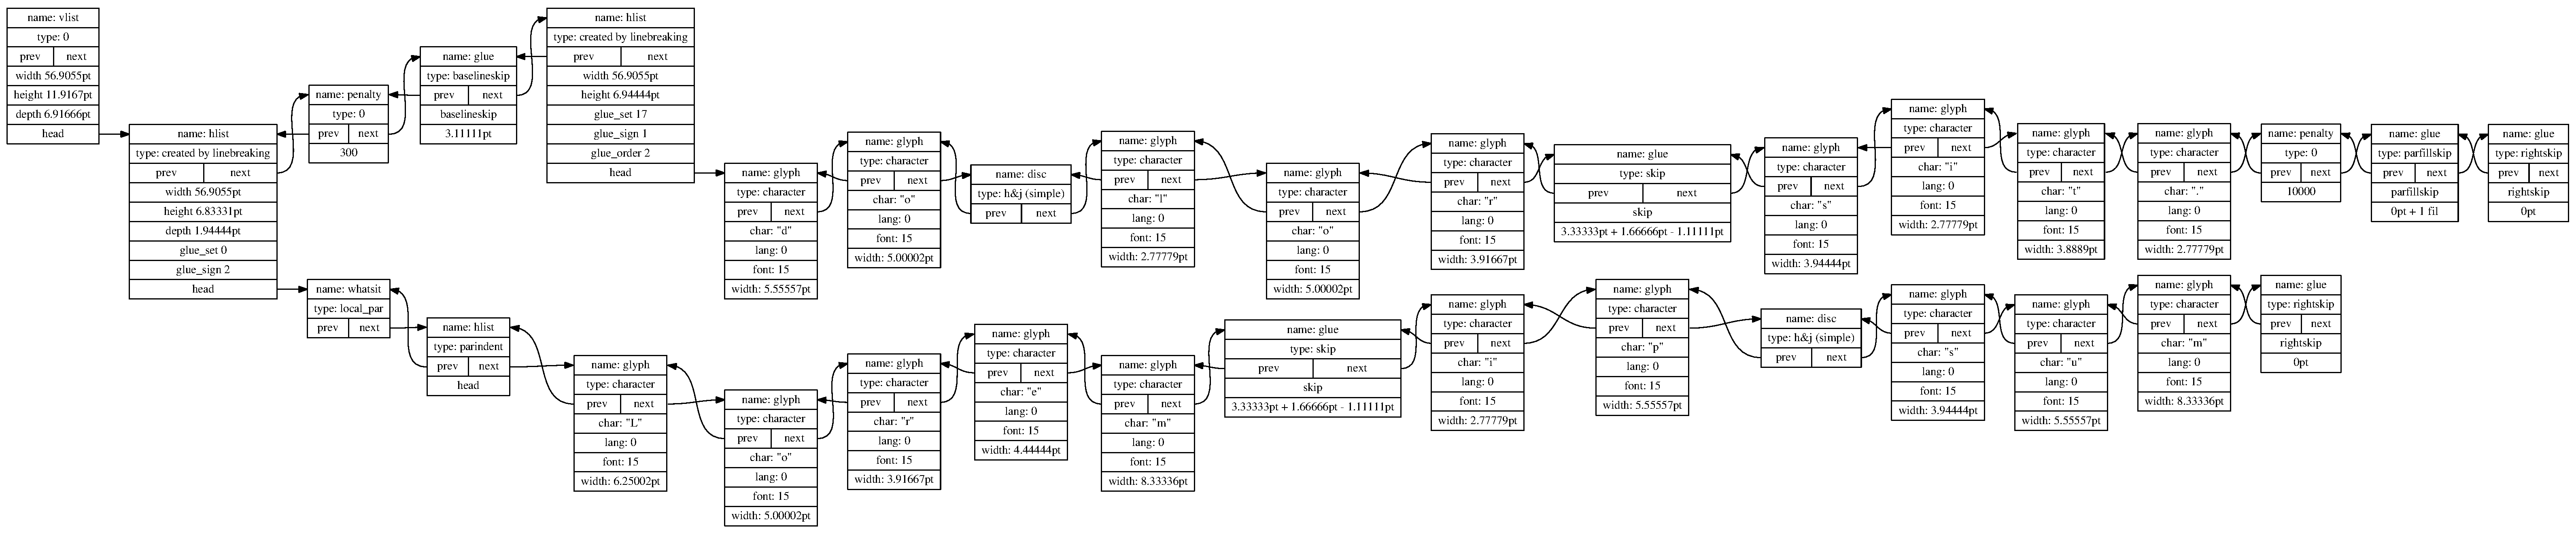
\includegraphics[width=\linewidth]{graphics/par}

\subsection{Tabular environment}

\noindent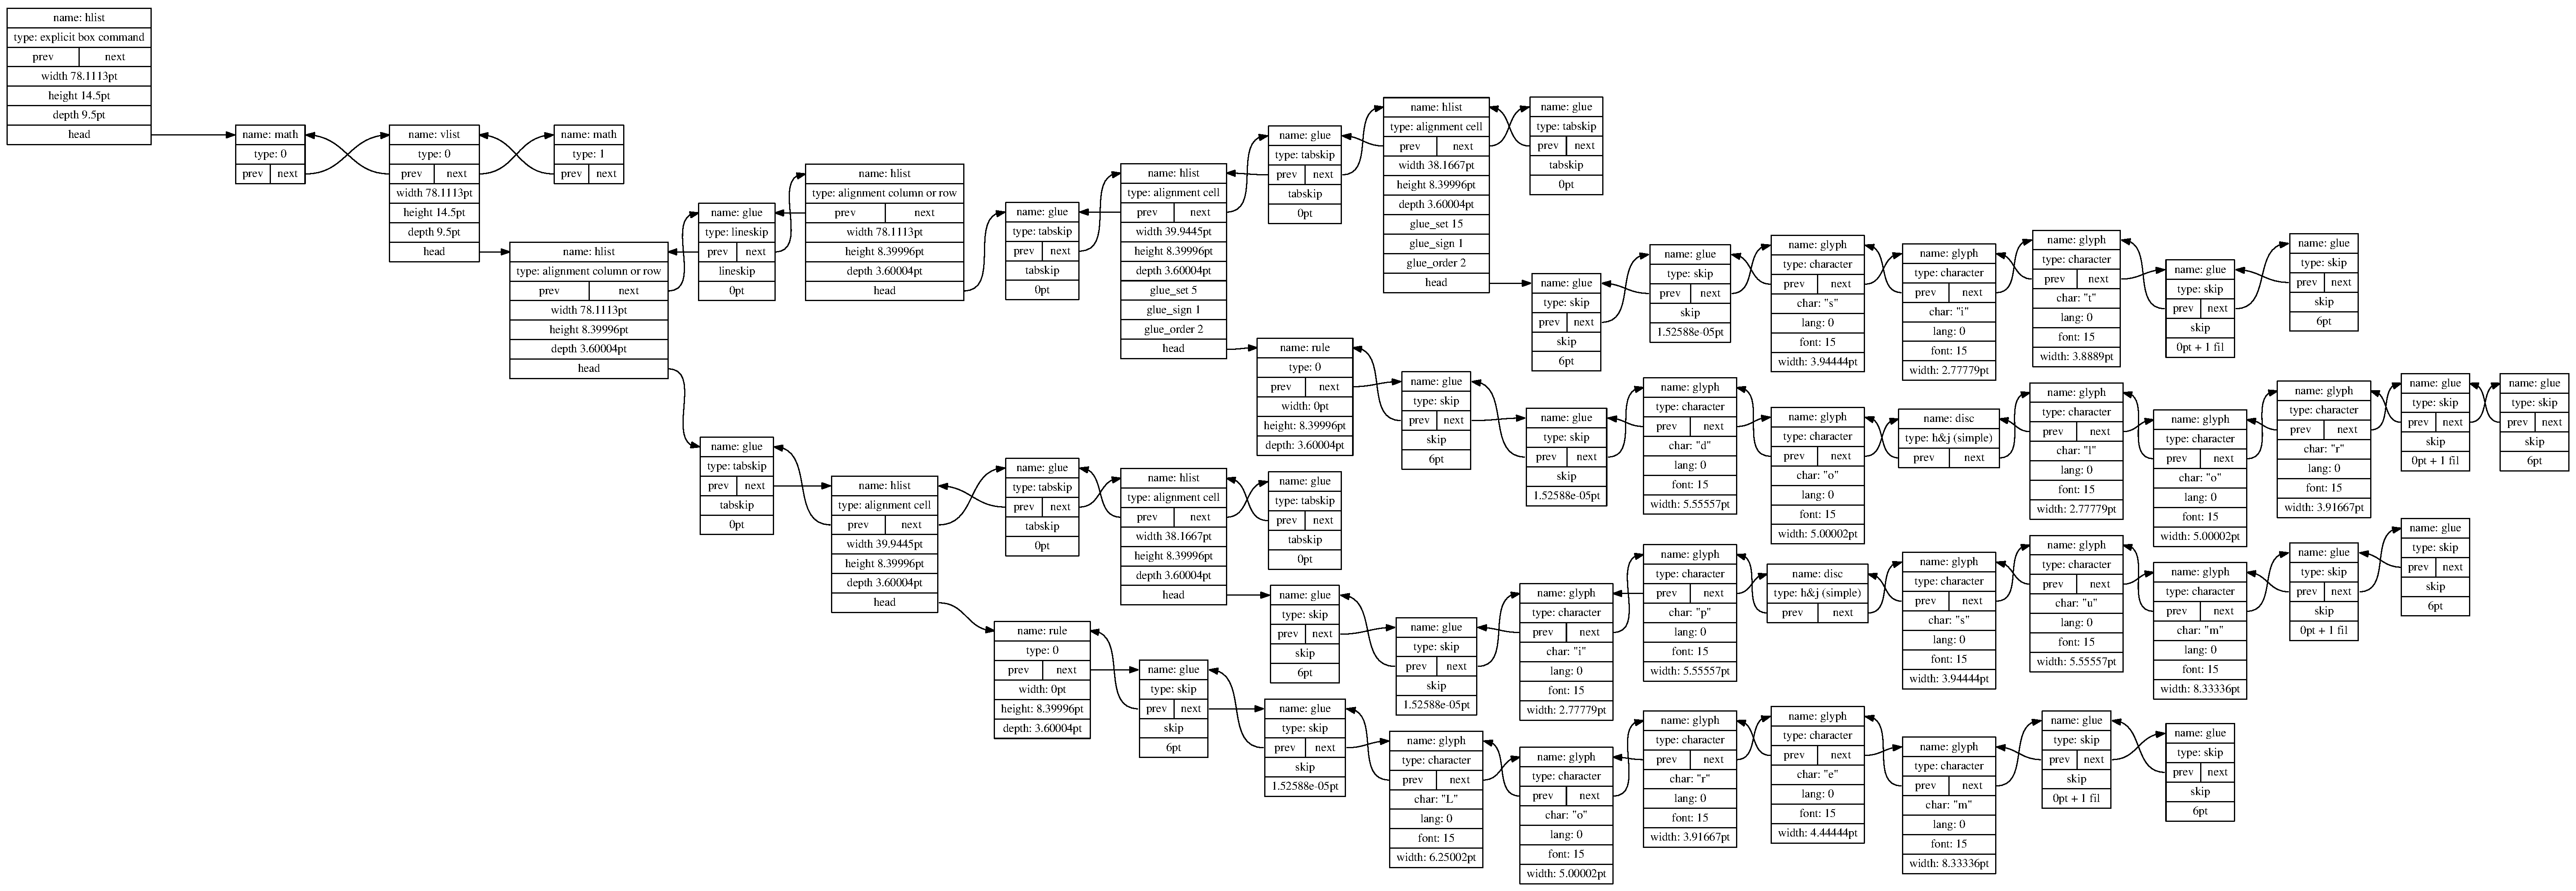
\includegraphics[width=\linewidth]{graphics/tabular}

\subsection{Picture environment}

\noindent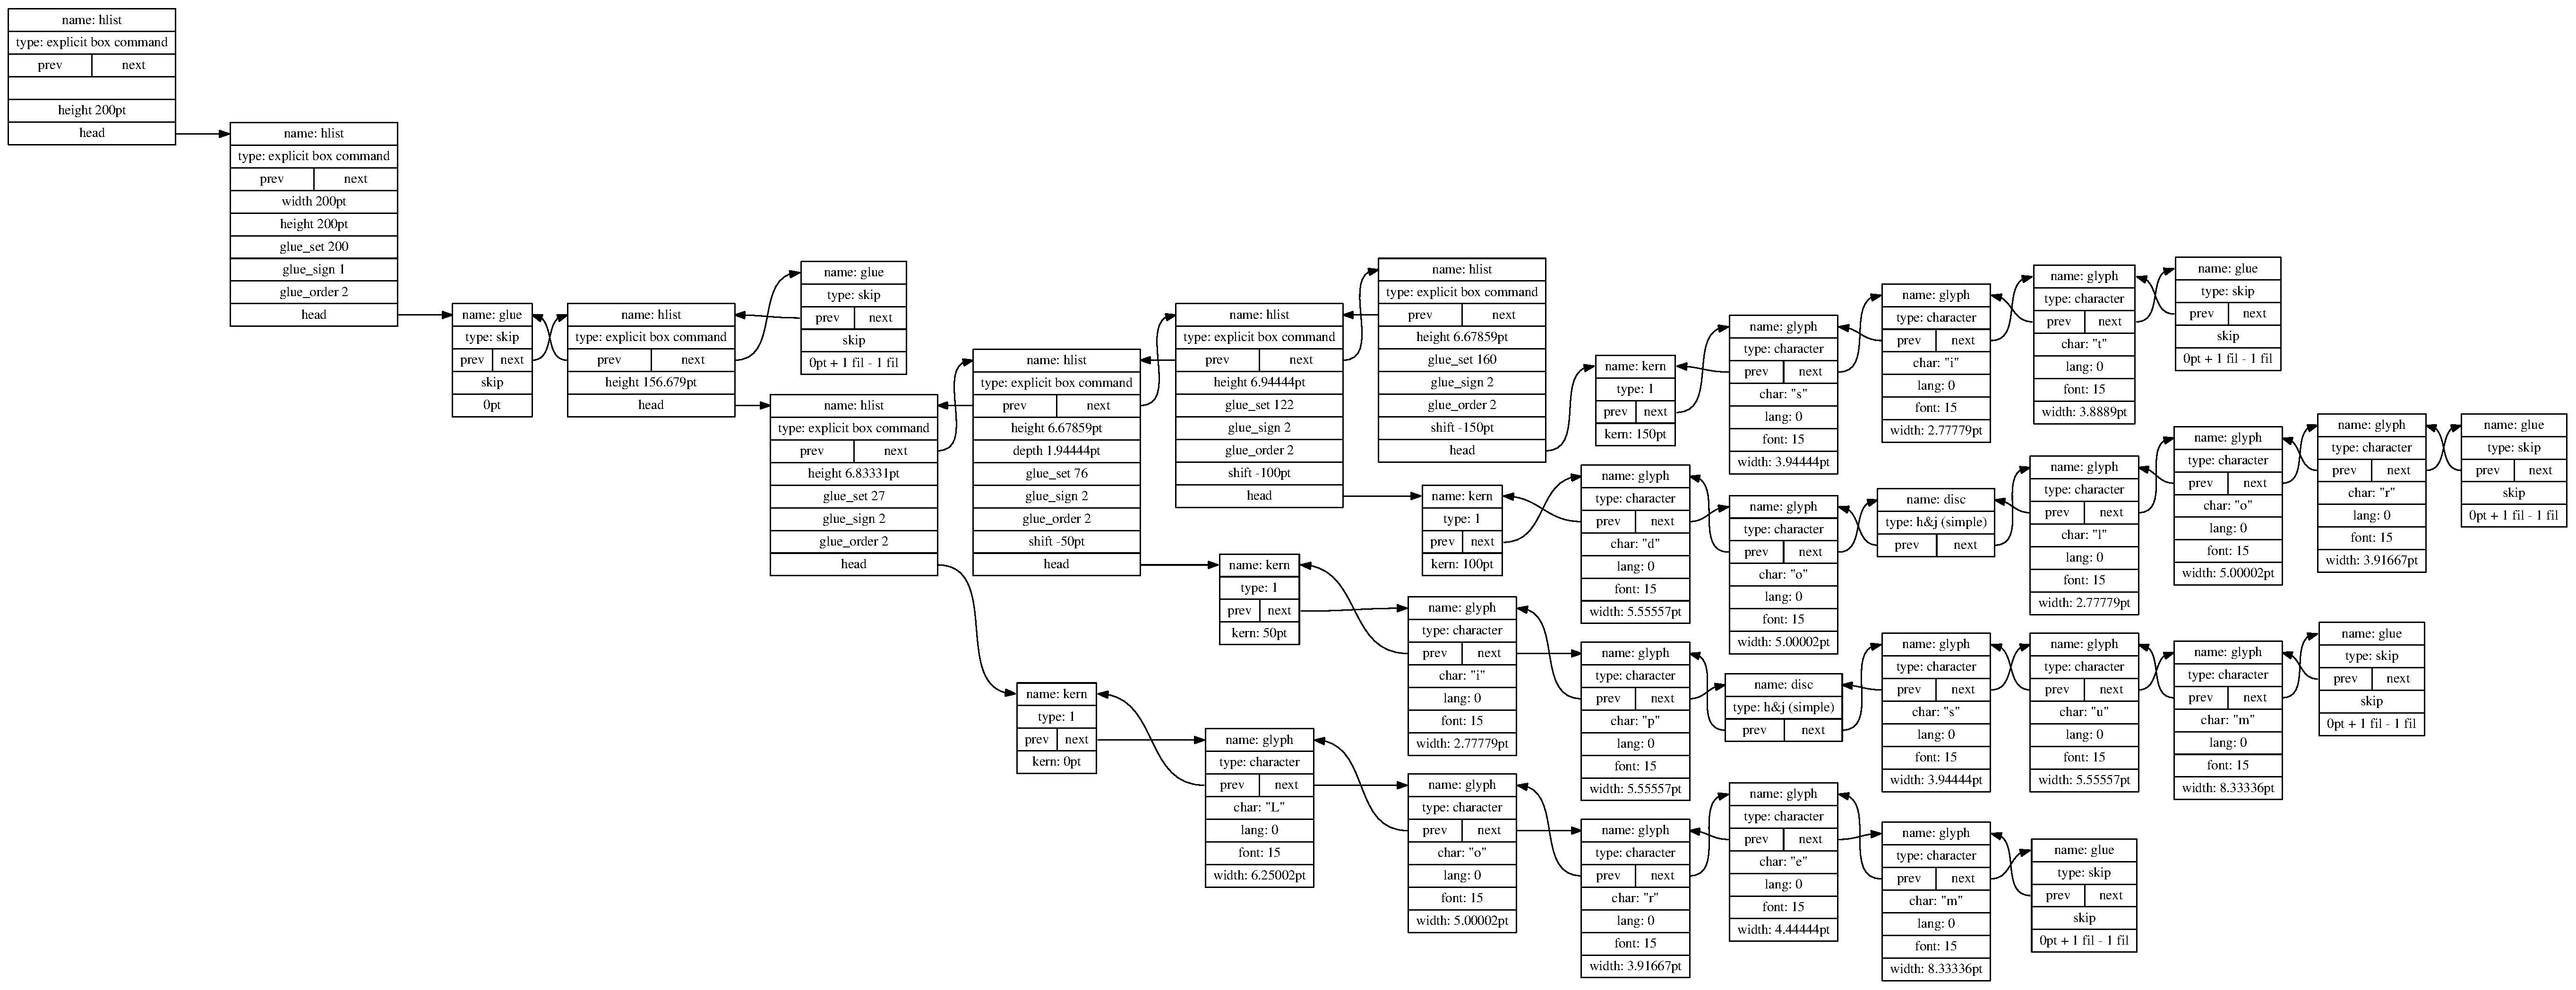
\includegraphics[width=\linewidth]{graphics/picture}

\DocInput{cloze.dtx}

\subsection{The file cloze.lua}

\inputminted{lua}{cloze.lua}

\pagebreak
\PrintChanges
\pagebreak
\PrintIndex
\end{document}
